\subsection{Problem 1. Model selection from data}
A quantity $Q(t)$ is measured at different times $t$ (in hours), and the following data are recorded:

\begin{center}
\begin{tabular}{c|ccccc}

$t$ & 0 & 1 & 2 & 3 & 4 \\
\hline
$Q(t)$ & 100 & 80 & 64 & 51.2 & 40.96 \\

\end{tabular}
\end{center}

\begin{enumerate}[label=(\alph*)]
    \item By looking at ratios between successive values, decide whether a linear or an exponential model is more appropriate for this data. Explain your reasoning clearly.
    \item Assuming an exponential model $Q(t) = Q_{0}a^{t}$, determine the parameters $Q_{0}$ and $a$. Then rewrite the model in the form $Q(t) = Q_{0}e^{kt}$ and find $k$.
    \item Using your model, estimate the time $t$ when $Q(t)$ will first fall below 20. Comment on how sensitive your answer is to small changes in the data.
    \item Discuss at least two limitations of using this exponential model for very large $t$ (e.g., $t \gg 4$). In what real-world situation could such a model be reasonable, and when would it break down?
\end{enumerate}

\subsection*{Strategy}
\subsection*{Solution}
\begin{enumerate}[label=(\alph*)]
    \item \textbf{Model Selection} \\
    To determine the appropriate model, we check for constant differences (linear) or constant ratios (exponential).
    
    \textbf{Check for Linear (Differences):}
    \begin{itemize}
        \item $80 - 100 = -20$
        \item $64 - 80 = -16$
    \end{itemize}
    The differences are not constant, so it is \textbf{not linear}.
    
    \textbf{Check for Exponential (Ratios):}
    \begin{itemize}
        \item $80 / 100 = 0.8$
        \item $64 / 80 = 0.8$
        \item $51.2 / 64 = 0.8$
    \end{itemize}
    Since the ratio between successive terms is constant ($0.8$), an \textbf{exponential model} is appropriate.

    \item \textbf{Determining Parameters} \\
    We assume the form $Q(t) = Q_{0}a^{t}$.
    \begin{itemize}
        \item $Q_{0}$ is the initial value at $t=0$, so $\mathbf{Q_{0} = 100}$.
        \item $a$ is the constant ratio found in part (a), so $\mathbf{a = 0.8}$.
    \end{itemize}
    The model is: 
    \[ Q(t) = 100(0.8)^{t} \]
    
    To rewrite as $Q(t) = Q_{0}e^{kt}$, we solve for $k$:
    \[ e^k = 0.8 \implies k = \ln(0.8) \approx -0.2231 \]
    The continuous decay model is:
    \[ \mathbf{Q(t) = 100e^{-0.2231t}} \]

    \item \textbf{Estimation and Sensitivity} \\
    We need to find $t$ when $Q(t) < 20$.
    \[ 20 = 100(0.8)^{t} \]
    \[ 0.2 = 0.8^{t} \]
    Taking the natural log of both sides:
    \[ \ln(0.2) = t \cdot \ln(0.8) \]
    \[ t = \frac{\ln(0.2)}{\ln(0.8)} \approx \frac{-1.6094}{-0.2231} \approx \mathbf{7.21 \text{ hours}} \]
    
    \textbf{Sensitivity Comment:} The calculation involves logarithms of ratios. A very small change in the data (e.g., if the ratio was $0.81$ instead of $0.8$) would change the denominator $\ln(a)$, leading to a significantly different time estimate. Thus, the prediction is quite sensitive to measurement noise in the original data.

    \item \textbf{Limitations for Large $t$} \\
    For very large $t$ (long term), the mathematical model has limitations:
    \begin{itemize}
        \item \textbf{The "Zero" Limit:} Mathematically, $Q(t)$ approaches 0 but never reaches it. In reality, if $Q(t)$ represents a physical substance (like atoms or bacteria), it is discrete. Eventually, you cannot have $0.01$ of an atom; the model breaks down when $Q(t) < 1$.
        \item \textbf{Changing Conditions:} The model assumes the decay rate $k$ is constant forever. In real-world biological or chemical systems, environmental conditions (temperature, pressure, metabolism) often change over long periods, altering the rate.
    \end{itemize}
    
    \textbf{Real-world context:} This is reasonable for \textbf{radioactive decay} (where physics dictates a constant rate) or \textbf{drug clearance} in the bloodstream. It breaks down when the concentration becomes so low that it is undetectable or interacts with background noise.

\end{enumerate}

\vspace{1cm}
\noindent\textbf{Visualizing the Decay:}

\begin{center}
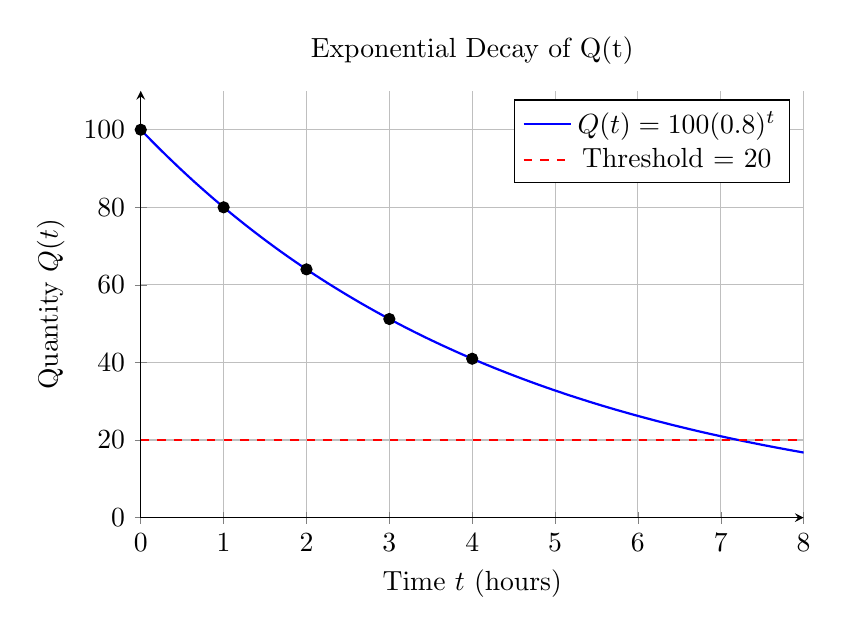
\begin{tikzpicture}
\begin{axis}[
    title={Exponential Decay of Q(t)},
    xlabel={Time $t$ (hours)},
    ylabel={Quantity $Q(t)$},
    axis lines=left,
    grid=major,
    domain=0:8,
    samples=100,
    width=10cm, height=7cm,
    ymin=0, ymax=110
]
\addplot[color=blue, thick] {100 * 0.8^x};
\addlegendentry{$Q(t) = 100(0.8)^t$}

\addplot[color=red, dashed] coordinates {(0,20) (8,20)};
\addlegendentry{Threshold = 20}

\addplot[
    color=black,
    mark=*,
    only marks
    ]
    coordinates {
    (0,100)(1,80)(2,64)(3,51.2)(4,40.96)
    };
\end{axis}
\end{tikzpicture}
\end{center}
\pagebreak
